\chapter{METHODOLOGY}
\onehalfspacing
\label{chap:methodology}
\vspace{-3em}
This qualitative research aims to use natural language processing (NLP) techniques to detect Borderline Personality Disorder (BPD) from user-generated text responses. To effectively detect BPD from user-generated text responses, our proposed methodology integrates transformer-based language models with a robust ensemble learning strategy.The research is divided into four phases - \textbf{Phase 1 : Dataset Collection , Phase 2 : Preprocessing, Phase 3: Model Training and Finetuning and Phase 4 : Explanation using Explainable AI.}

The pipeline initiates with phase 1 , where the data is collected through structured questionnaires to elicit text responses relevant to psychological patterns associated with BPD . And from those data , a dataset was created by the experts. 

In phase 2 , the collected data undergoes extensive preprocessing includings cleaning , normalization , tokenization and embedding preparation using word embedding models like TfIDF , Word2vec , Glove , Fasttext etc. This phase ensures that the response is ready for NLP modeling. 

In phase 3 , a diverse set of transformer-based models(such as BERT , RoBERTa , ELECTRA , DistilBERT ) are selected and fine-tuned on the preprocessed dataset . Two parallel modeling strategies are applied : 1. Training Individual Transformer Models and 2. Ensemble Learning Approach, which aggregates the multiple finetuned models through techniques like majority voting , stacing , weighted average , bagging , boosting to  improve accuracy, stability, and generalizability.

Finally phase 4 introduces an explainability layer using state-of-art XAI methods such as LIME. LIME provides interpretable insights into the model's decision-making process by identifying key words, phrases or linguistic features contributing to the BPD detection. The integration of XAI ensures ethical transparency and supports mental health professionals in understanding AI-driven assessments.

\begin{figure}
    \centering
    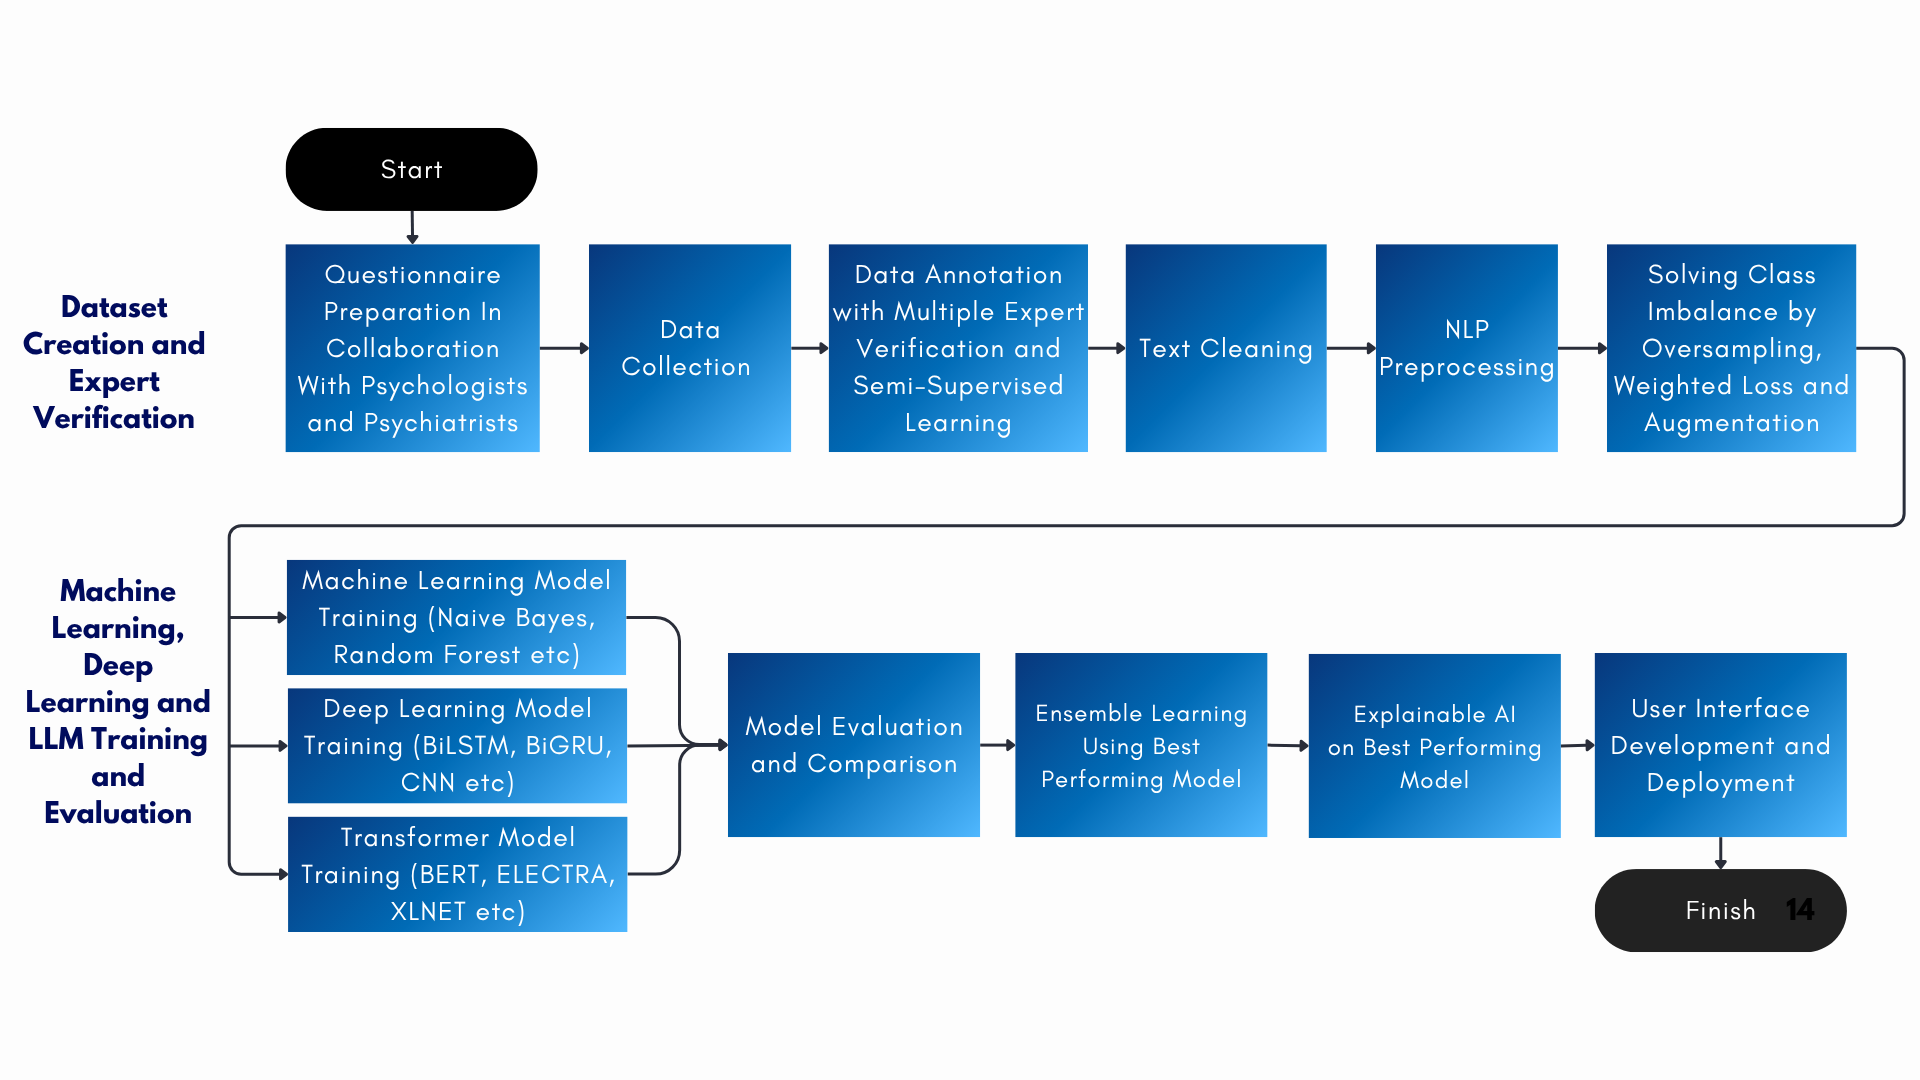
\includegraphics[width=\linewidth, height=10cm]{new figures/methodology.png}
    \caption{Research Methodology}
    \label{fig:methodology}
\end{figure}

Figure \ref{fig:methodology} illustrates the research methodology followed in this study. The key steps in the research, including dataset creation, detailed comparative analysis of machine learning, deep learning and transformer models, screening tool deployment with explainable AI, have been shown. 

%%Marked , See the ss from laptop

\section{Dataset collection}
\subsection{Data Sources}
As the primary objective of this research is the detection of Borderline Personality Disorder (BPD) from user-generated text responses, the acquisition of high-quality, contextually relevant data was prioritized as the foundational phase of the study. Existing public datasets related to mental health disorder detection are predominantly derived from social media platforms (such as Reddit or Twitter) or rating-based self-assessment scales. However, these sources often lack clinical validity and pose challenges for accurate natural language processing (NLP) applications.
Social media content, in particular, tends to be informal, contextually ambiguous, and often written for entertainment or social engagement, rather than as a genuine reflection of the user's psychological state. Consequently, such data may not reliably indicate mental health symptoms or patterns associated with BPD, leading to noisy inputs and compromised model performance in clinical or diagnostic NLP tasks.
To address this limitation, this research emphasizes direct data collection through structured questionnaires based on the Diagnostic and Statistical Manual of Mental Disorders (DSM-5), designed to elicit emotionally and psychologically meaningful text responses. This approach ensures that the data is task-specific, context-aware, and ethically sound, providing a more reliable foundation for subsequent NLP modeling and BPD detection
Following expert consultation, a custom questionnaire was developed with the help of these domain specialists. The questionnaire was carefully crafted to map to the DSM-5 diagnostic criteria for BPD \cite{APA2013}, focusing particularly on:
\begin{enumerate}
    \item \textbf{Criterion A} (identity disturbance and interpersonal instability), captured through nine open-ended, natural language questions.
     \item \textbf{Criteria B to F} (covering impulsivity, affective instability, self-harm, etc.), assessed through five dichotomous (Yes/No) questions. 
\end{enumerate}

\subsection{Dataset Description}
The survey was administered to a diverse group of 362 participants, each of whom responded to:
nine open-ended natural language questions aimed at assessing Criterion A (identity disturbance and interpersonal dysfunction) and five dichotomous (Yes/No) questions covering Criteria B to F, such as affective instability, impulsivity, self-harm, chronic feelings of emptiness, and dissociation. 
This resulted in a total of 3,258 QnA pairs (362 participants × 9 questions), forming the core dataset for NLP modeling. These responses were collected specifically to enable the development of a diagnostic screening system and are significantly more task-specific and clinically grounded than data derived from informal or recreational online platforms. 

\subsection{Data Annotation}
The annotation process was critical to transforming the raw textual data into a labeled dataset suitable for supervised machine learning tasks. Each QnA pair was labeled according to the presence or absence of indications of BPD-related traits. The possible labels were defined as follows:
\begin{enumerate}
    \item \textbf{0 = Normal:} No clear signs or textual evidence of BPD symptoms.
    \item \textbf{1 = BPD:} Textual indicators suggest the presence of symptoms consistent with BPD, according to DSM-5 criteria.
    \item \textbf{2 = Inconclusive:} The response was ambiguous, lacked sufficient detail, or was contradictory, making a definitive classification uncertain.
\end{enumerate}

To ensure both quality and efficiency in annotation, the process was conducted in two stages. First stage was manual annotation by domain experts of the first half of the dataset. Subsequently, the second stage was semi-supervised annotation with expert verification.

\subsubsection{Stage 1 : Manual Annotation by Domain Experts}
The dataset was first divided into two equal halves. The first half (1,629 QnA pairs) was manually annotated by a team of three mental health professionals (two psychologists and one psychiatrist). Each expert independently reviewed and labeled the responses. In cases where the experts disagreed on the label, the relevant QnA pairs were flagged for re-evaluation. These instances were then discussed collaboratively until a consensus was reached, ensuring a high degree of annotation reliability and clinical validity.

\subsubsection{Stage 2 : Semi-Supervised Annotation with Expert Verification}
To expedite the labeling process while maintaining accuracy, the first half of the manually labeled dataset was used to train a semi-supervised learning model. This model was employed to predict labels for the remaining half of the dataset. The auto-labeled data was not accepted as-is; instead, it underwent a verification process by the same three experts who reviewed and corrected the machine-generated labels where necessary. Discrepancies in this phase were also resolved via consensus.

This two-stage annotation strategy allowed the research to combine the rigor of expert-driven labeling with the efficiency of machine-assisted annotation, resulting in a fully labeled dataset that is both clinically sound and scalable for model training.

\section{Data Pre-processing}
Before applying any machine learning or deep learning techniques, the raw textual data collected from participants underwent a comprehensive preprocessing pipeline to ensure its suitability for natural language processing (NLP) tasks. This step was essential to reduce noise, improve consistency, and enhance the overall quality of the data, thereby allowing models to learn meaningful patterns relevant to BPD detection.

\subsection{Data Cleaning}
The initial phase of preprocessing involved the removal of irrelevant or meaningless entries that could negatively impact model performance for the machine learning and deep learning models. These included:
\begin{enumerate}
    \item Repetitive or non-alphabetic characters such as "....................", "nnnnnnnnnnnnnn", and other similar noise patterns.

     \item Responses that contained only emojis, keyboard mashing, or placeholder text with no semantic content.

    \item Excessive punctuation , special symbols , non-informative symbols that lacked contextual value.
\end{enumerate}
This cleaning step helped to eliminate input artifacts and preserved only those responses that carried potential psychological indicators.

\subsection{Text Normalization}
The text normalization process consisted of several subtasks:
\begin{enumerate}
    \item \textbf{Contraction Expansion:} Common contractions (e.g., "I'm", "can't", "won't") were expanded to their full forms ("I am", "cannot", "will not") to maintain consistency and clarity.
    \item \textbf{Slang Removal and Replacement:} Informal slang words were either removed or replaced with their standard equivalents using a curated slang-to-standard dictionary, ensuring that model interpretation aligned with clinically relevant vocabulary.
    \item \textbf{Lowercasing:} All text was converted to lowercase to avoid redundant vocabulary and simplify tokenization. 
\end{enumerate}
This text normalization process is also a part of the machine learning , deep learning and transformer models. 

\subsection{Text Pre-processing for Machine Learning and Deep Learning}
Text preprocessing is a crucial step in any natural language processing (NLP) task, particularly in the context of detecting psychological disorders such as Borderline Personality Disorder (BPD). In this research, the preprocessing pipeline was meticulously designed to convert raw user-generated responses into clean, standardized, and semantically meaningful formats suitable for various modeling techniques, including traditional machine learning, deep learning, and transformer-based approaches. The preprocessing process involved several stages, as outlined below:

\subsubsection{Question-Answer Pair Construction} 
The raw dataset comprised responses from 362 participants, each answering nine open-ended questions targeting Criterion A of BPD as per DSM-5. These responses were structured into Question-Answer (QnA) pairs, where each answer was paired with its corresponding prompt. Each QnA pair was treated as an individual sample for training and evaluation.

\subsubsection{Tokenization}
Each cleaned and normalized text sample was broken into individual tokens (words or subwords) using tokenizer tools appropriate for the subsequent model. Tokenization served as the foundation for embedding and vectorization steps.

\subsubsection{Stop Word Removal and Frequent Word Filtering}
\textbf{Stop Words} Commonly occurring function words (e.g., "the", "is", "and") that do not contribute significant semantic value were removed using standard stop word lists (e.g., NLTK or SpaCy).

\textbf{Frequent/Redundant Words} Words that appeared excessively across nearly all responses but carried limited diagnostic information were identified and removed to reduce feature noise.

\subsubsection{Lemmatization}
To normalize word forms, lemmatization was applied. This process converts words to their base or dictionary form (e.g., "running" → "run", "better" → "good"), which helped unify variations of the same word and improve the efficiency of token-level feature extraction. Lemmatization preserved the correct meaning better than stemming, making it more suitable for clinical text.

\subsubsection{Feature Extraction Techniques}
Depending on the modeling technique (machine learning, deep learning), different vectorization and embedding strategies were used to convert the text into numerical features:
\begin{enumerate}

    \item \textbf{TF-IDF (Term Frequency–Inverse Document Frequency):} For traditional machine learning models (e.g., Logistic Regression, SVM), the text was converted into sparse vectors using TF-IDF. This method captured the importance of words in a document relative to the overall corpus, allowing the model to focus on diagnostically informative terms.
    \item \textbf{Word Embeddings :} For deep learning models such as LSTM and BiLSTM, word embeddings were used to provide dense, low-dimensional representations of words:
    \item \textbf{Word2Vec:} Trained on a large corpus, this embedding captured semantic relationships using either CBOW or Skip-gram architectures.
    \item \textbf{GloVe (Global Vectors for Word Representation):} Pretrained vectors that learned word co-occurrence statistics from massive datasets (e.g., Wikipedia, Common Crawl).
    \item \textbf{FastText:} Enhanced word embeddings that included subword information, allowing for better handling of rare or misspelled words.
    \item \textbf{BERT:} Bidirectional Encoder Representations from Transformers (BERT) was used to generate token-level and sentence-level contextual embeddings, capable of capturing complex linguistic structures and psychological indicators.
    \item \textbf{Sentence Vectorization:} CLS token outputs or sentence embedding techniques were used to represent the entire response as a single dense vector.
\end{enumerate}
These embeddings were either used as fixed input or fine-tuned during model training and  significantly improved the model’s ability to understand context, emotion, and diagnostic cues within the text.

\subsection{Text Preprocessing for Large Language Models}
Large language models such as BERT, RoBERTa, and DistilBERT have transformed natural language processing by providing deep contextual understanding of text. However, the performance of these models still heavily depends on the quality of the input data. Therefore, a structured and task-specific preprocessing pipeline was applied to prepare the user-generated text responses for fine-tuning transformer-based architectures in this research. The following steps outline the full pipeline used:

\begin{enumerate}
    \item \textbf{Question-Answer Pair Construction} : Each participant responded to a set of open-ended questions based on Criterion A of the DSM-5 for BPD. These responses were combined with their respective prompts to form complete question-answer (QnA) pairs, providing essential context for the user’s reply. 

    \item \textbf{Tokenization} : Transformer models use specific tokenizers based on subword segmentation techniques (e.g., WordPiece or Byte-Pair Encoding). Each text sample (QnA pair) was tokenized using the appropriate tokenizer for the model architecture.     
\end{enumerate}

\section{Model Training and Finetuning}
In this section , the preprocessing of the dataset and the parameter finetuning are described that has been used in the research .  
\subsection{Dataset Preparation}
\subsubsection{Dataset Preparation for Machine Learning Model and Deep Learning}
To ensure robust model training and fair evaluation, the dataset was carefully split and balanced using stratification and augmentation techniques:

\begin{enumerate}
    \item \textbf{Stratified Splitting by Question ID and Label}
    \begin{itemize}
        \item \textbf{Question-wise Stratification:} QnA pairs were split such that each training, validation, and testing set maintained a consistent distribution of question IDs. This preserved the structural balance of the dataset by ensuring that every split contained a proportionate number of responses for each of the nine DSM-5-based open-ended questions.

        \item \textbf{Label-wise Stratification:}Simultaneously, stratification based on class labels (0 = Normal, 1 = BPD, 2 = Inconclusive) was applied. This ensured that each split contained an approximately equal proportion of all classes, which is crucial for unbiased model evaluation and generalization.
    \end{itemize}
    \item \textbf{Handling Class Imbalance}
    The initial label distribution revealed a significant imbalance, with the majority of instances labeled as 0 (Normal). To address this, the following techniques were employed:
    \begin{itemize}
        \item \textbf{Oversampling Techniques:}
            \textbf{SMOTE (Synthetic Minority Over-sampling Technique)} and \textbf{ADASYN (Adaptive Synthetic Sampling)} were applied to the training set to synthetically generate new samples for minority classes (labels 1 and 2), thereby balancing the dataset.
        
        
        \item \textbf{Textual Data Augmentation:}
        \textbf{Augmentation} techniques such as synonym replacement, paraphrasing, and back translation were used to increase the sample size of underrepresented classes (1 and 2) until they matched the majority class (label 0).
        These augmented samples were carefully reviewed to maintain semantic validity and emotional coherence in responses.

    \end{itemize}
\end{enumerate}


\subsubsection{Dataset Preparation for Large Language Models}
Due to the inherent complexity and contextual sensitivity of transformer-based language models, a tailored approach was adopted to address the dataset’s class imbalance without relying on oversampling methods that could introduce redundancy or overfitting. The following strategies were implemented:

\begin{enumerate}
    \item \textbf{Class Weight Loss Function}
    \begin{itemize}
        \item Rather than modifying the data distribution, transformer models were trained using a class-weighted cross-entropy loss function. This approach involved assigning higher penalty weights to the minority classes (label 0 = Normal, label 1 = BPD, label 2 = Inconclusive) during model optimization.The loss function dynamically adjusts the contribution of each class in proportion to its inverse frequency in the training set, ensuring that misclassifying a minority class sample results in a higher loss.
    \end{itemize}

    \item \textbf{Dataset Augmentation}
    \begin{itemize}
        \item Similar augmentation techniques as used in ML/DL were applied to increase the diversity and quantity of samples in the minority classes, enhancing the model's exposure to varied linguistic representations of BPD symptoms
    \end{itemize}
\end{enumerate}

\subsection{Experimental Setup}
\subsubsection{Experimental Setup for Machine Learning Model}

\begin{center}
\small
\begin{longtable}{|l|l|l|l|}
\caption{Model Configurations with Feature Extraction and Hyperparameters}
\label{tab:model_config} \\

\hline
\textbf{Model} & \textbf{Feature Extraction} & \textbf{Class Balancing Technique} & \textbf{Hyperparameters} \\ 
\hline
\endfirsthead

\multicolumn{4}{c}%
{{\textbf{\tablename\ \thetable{}} continued from previous page}} \\
\hline
\textbf{Model} & \textbf{Feature Extraction} & \textbf{Class Balancing Technique} & \textbf{Hyperparameters} \\
\hline
\endhead

\hline
\endfoot

\hline
\endlastfoot

\multirow{5}{*}{LSVM} & TFIDF & \multirow{5}{*}{\parbox{3cm}{SMOTE\\ADASYN\\Text Augmentation}} & \\ \cline{2-2}
& Word2Vec & & C=1.0 \\ \cline{2-2}
& Glove & & kernel=linear \\ \cline{2-2}
& Fasttext & & max\_iter=2000 \\ \cline{2-2}
& BERT Embeddings & &  \\ \hline

\multirow{5}{*}{LR} & TFIDF & \multirow{5}{*}{\parbox{3cm}{SMOTE\\ADASYN\\Text Augmentation}} & \\ \cline{2-2}
& Word2Vec & & C=0.9 \\ \cline{2-2}
& Glove & & penalty=l2\\ \cline{2-2}
& Fasttext & & solver=liblinear \\ \cline{2-2}
& BERT Embeddings & & \\ \hline

\multirow{5}{*}{NB} & TFIDF & \multirow{5}{*}{\parbox{3cm}{SMOTE\\ADASYN\\Text Augmentation}} & \\ \cline{2-2}
& Word2Vec & & fit\_prior=False \\ \cline{2-2}
& Glove & & alpha=1.5 \\ \cline{2-2}
& Fasttext & & \\ \cline{2-2}
& BERT Embeddings & & \\ \hline

\multirow{5}{*}{KNN} & TFIDF & \multirow{5}{*}{\parbox{3cm}{SMOTE\\ADASYN\\Text Augmentation}} & \\ \cline{2-2}
& Word2Vec & & n\_neighbors=7 \\ \cline{2-2}
& Glove & & weights=distance \\ \cline{2-2}
& Fasttext & & algorithm=brute \\ \cline{2-2}
& BERT Embeddings & &  \\ \hline
\newpage
\multirow{5}{*}{DT} & TFIDF & \multirow{5}{*}{\parbox{3cm}{SMOTE\\ADASYN\\Text Augmentation}} & \\ \cline{2-2}
& Word2Vec & & criterion=entropy \\ \cline{2-2}
& Glove & & max\_depth=12 \\ \cline{2-2}
& Fasttext & & min\_samples\_leaf=1 \\ \cline{2-2}
& BERT Embeddings & &  \\ \hline

\multirow{5}{*}{RF} & TFIDF & \multirow{5}{*}{\parbox{3cm}{SMOTE\\ADASYN\\Text Augmentation}} & \\ \cline{2-2}
& Word2Vec & & n\_estimators=120 \\ \cline{2-2}
& Glove & & max\_depth=25 \\ \cline{2-2}
& Fasttext & & bootstrap=False \\ \cline{2-2}
& BERT Embeddings & &  \\ \hline

\multirow{5}{*}{XGB} & TFIDF & \multirow{5}{*}{\parbox{3cm}{SMOTE\\ADASYN\\Text Augmentation}} & \\ \cline{2-2}
& Word2Vec & & learning\_rate=0.05 \\ \cline{2-2}
& Glove & & gamma=0.3 \\ \cline{2-2}
& Fasttext & & subsample=0.8 \\ \cline{2-2}
& BERT Embeddings & &  \\ \hline

% --- break here before page overflows ---

\multirow{2}{*}{LGBM} & TFIDF & \multirow{5}{*}{\parbox{3cm}{SMOTE\\ADASYN\\Text Augmentation}} & \\ \cline{2-2}
& Word2Vec & & learning\_rate=0.1 \\ \cline{1-2} \cline{4-4}
\multirow{3}{*}{LGBM} & Glove & & num\_leaves=25 \\ \cline{2-2} \cline{4-4}
& Fasttext & & boosting=goss \\ \cline{2-2} \cline{4-4}
& BERT Embeddings & & \\ \hline


\multirow{5}{*}{AdaBoost} & TFIDF & \multirow{5}{*}{\parbox{3cm}{SMOTE\\ADASYN\\Text Augmentation}} & \\ \cline{2-2}
& Word2Vec & & n\_estimators=60 \\ \cline{2-2}
& Glove & & learning\_rate=1.2 \\ \cline{2-2}
& Fasttext & & algorithm=SAMME \\ \cline{2-2}
& BERT Embeddings & &  \\ \hline

\end{longtable}
\end{center}

\newpage
\subsubsection{Experimental Setup for Deep Learning}


\begin{longtable}[H]{|l|l|p{2.5cm}|p{4cm}|}
\caption{Model Configuration For Oversampling Technique} \\
\hline
\textbf{Models} & \textbf{Feature Extractions} & \textbf{Class Balancing} & \textbf{HyperParameter} \\ \hline
\endfirsthead
\hline
\textbf{Models} & \textbf{Feature Extractions} & \textbf{Class Balancing} & \textbf{HyperParameter} \\ \hline
\endhead

\multirow{6}{*}{GRU} & \multirow{2}{*}{Word2Vec} & \multirow{6}{2.5cm}{\raggedright SMOTE \\ ADASYN} & \multirow{6}{4cm}{\raggedright Output\_dim = 300\\ Learning Rate = 5e-4\\ Weight\_decay = 1e-5\\ Dropout = 0.2\\ Patience = 3\\ Epoch = 30} \\
 & & & \\ \cline{2-2}
 & \multirow{2}{*}{Glove} & & \\
 & & & \\ \cline{2-2}
 & \multirow{2}{*}{Fasttext} & & \\
 & & & \\ \hline

\multirow{6}{*}{BiGRU} & \multirow{2}{*}{Word2Vec} & \multirow{6}{2.5cm}{\raggedright SMOTE \\ ADASYN} & \multirow{6}{4cm}{\raggedright Output\_dim = 300\\ Learning Rate = 5e-4\\ Weight\_decay = 1e-5\\ Dropout = 0.2\\ Patience = 3\\ Epoch = 30} \\
 & & & \\ \cline{2-2}
 & \multirow{2}{*}{Glove} & & \\
 & & & \\ \cline{2-2}
 & \multirow{2}{*}{Fasttext} & & \\
 & & & \\ \hline

\multirow{6}{*}{LSTM} & \multirow{2}{*}{Word2Vec} & \multirow{6}{2.5cm}{\raggedright SMOTE \\ ADASYN} & \multirow{6}{4cm}{\raggedright Output\_dim = 300\\ Learning Rate = 5e-4\\ Weight\_decay = 1e-5\\ Dropout = 0.2\\ Patience = 3\\ Epoch = 30} \\
 & & & \\ \cline{2-2}
 & \multirow{2}{*}{Glove} & & \\
 & & & \\ \cline{2-2}
 & \multirow{2}{*}{Fasttext} & & \\
 & & & \\ \hline

\multirow{6}{*}{BiLSTM} & \multirow{2}{*}{Word2Vec} & \multirow{6}{2.5cm}{\raggedright SMOTE \\ ADASYN} & \multirow{6}{4cm}{\raggedright Output\_dim = 300\\ Learning Rate = 5e-4\\ Weight\_decay = 1e-5\\ Dropout = 0.2\\ Patience = 3\\ Epoch = 30} \\
 & & & \\ \cline{2-2}
 & \multirow{2}{*}{Glove} & & \\
 & & & \\ \cline{2-2}
 & \multirow{2}{*}{Fasttext} & & \\
 & & & \\ \hline
 
\multirow{6}{*}{CNN} & \multirow{2}{*}{Word2Vec} & \multirow{6}{\linewidth}{\raggedright SMOTE \\ ADASYN} & \multirow{6}{\linewidth}{\raggedright Output\_dim = 300\\ Learning Rate = 5e-4\\ Weight\_decay = 1e-5\\ Dropout = 0.2\\ Patience = 3\\ Epoch = 30} \\
 & & & \\ \cline{2-2}
 & \multirow{2}{*}{Glove} & & \\
 & & & \\ \cline{2-2}
 & \multirow{2}{*}{Fasttext} & & \\
 & & & \\ 
\end{longtable}

% \vspace{1em}
\textbf{(2) Text Augmentation}
\begin{longtable}{|l|l|l|l|}
 \caption{Model Configuration For Text Augmentation} \\
\hline

\textbf{Models} & \textbf{Feature Extractions} & \textbf{Class Balancing} & \textbf{HyperParameter} \\ \hline
\endfirsthead
\hline
\textbf{Models} & \textbf{Feature Extractions} & \textbf{Class Balancing} & \textbf{HyperParameter} \\ \hline
\endhead

% GRU
\multirow{6}{*}{GRU} 
  & \multirow{2}{*}{Word2Vec} & \multirow{6}{*}{Text Augmentation} 
    & \multirow{6}{*}{%
      \shortstack[l]{%
        Output\_dim = 300\\
        Learning Rate = 3e-4\\
        Weight\_decay = 0.01\\
        Dropout = 0.2\\
        Patience = 5\\
        Epoch = 30%
      }%
    } \\
  & & & \\ 
  \cline{2-2}
  & \multirow{2}{*}{Glove} & & \\
  & & & \\
  \cline{2-2}
  & \multirow{2}{*}{Fasttext} & & \\
  & & & \\ \hline

% BiGRU
\multirow{6}{*}{BiGRU} 
  & \multirow{2}{*}{Word2Vec} & \multirow{6}{*}{Text Augmentation} 
    & \multirow{6}{*}{%
      \shortstack[l]{%
        Output\_dim = 300\\
        Learning Rate = 3e-4\\
        Weight\_decay = 0.01\\
        Dropout = 0.2\\
        Patience = 5\\
        Epoch = 30%
      }%
    } \\
  & & & \\ 
  \cline{2-2}
  & \multirow{2}{*}{Glove} & & \\
  & & & \\
  \cline{2-2}
  & \multirow{2}{*}{Fasttext} & & \\
  & & & \\ \hline

% LSTM
\multirow{6}{*}{LSTM} 
  & \multirow{2}{*}{Word2Vec} & \multirow{6}{*}{Text Augmentation} 
    & \multirow{6}{*}{%
      \shortstack[l]{%
        Output\_dim = 300\\
        Learning Rate = 3e-4\\
        Weight\_decay = 0.01\\
        Dropout = 0.2\\
        Patience = 5\\
        Epoch = 30%
      }%
    } \\
  & & & \\ 
  \cline{2-2}
  & \multirow{2}{*}{Glove} & & \\
  & & & \\
  \cline{2-2}
  & \multirow{2}{*}{Fasttext} & & \\
  & & & \\ \hline

% BiLSTM
\multirow{6}{*}{BiLSTM} 
  & \multirow{2}{*}{Word2Vec} & \multirow{6}{*}{Text Augmentation} 
    & \multirow{6}{*}{%
      \shortstack[l]{%
        Output\_dim = 300\\
        Learning Rate = 3e-4\\
        Weight\_decay = 0.01\\
        Dropout = 0.2\\
        Patience = 5\\
        Epoch = 30%
      }%
    } \\
  & & & \\ 
  \cline{2-2}
  & \multirow{2}{*}{Glove} & & \\
  & & & \\
  \cline{2-2}
  & \multirow{2}{*}{Fasttext} & & \\
  & & & \\ \hline

% CNN
\multirow{6}{*}{CNN} 
  & \multirow{2}{*}{Word2Vec} & \multirow{6}{*}{Text Augmentation} 
    & \multirow{6}{*}{%
      \shortstack[l]{%
        Output\_dim = 300\\
        Learning Rate = 3e-4\\
        Weight\_decay = 0.01\\
        Dropout = 0.2\\
        Patience = 5\\
        Epoch = 30%
      }%
    } \\
  & & & \\ 
  \cline{2-2}
  & \multirow{2}{*}{Glove} & & \\
  & & & \\
  \cline{2-2}
  & \multirow{2}{*}{Fasttext} & & \\
  & & & \\ \hline

\end{longtable}


\subsubsection{Experimental Setup for Large Language Model}

\begin{table}[H]
  \centering
  \begin{tabular}{|l|l|l|l|}
    \hline
    \textbf{Model} & \textbf{Feature Extraction} & \textbf{Class Balancing Technique} & \textbf{Hyperparameter} \\ \hline

    Electra &
    \begin{tabular}[c]{@{}l@{}}Electra\\Tokenizer\end{tabular} &
    \begin{tabular}[c]{@{}l@{}}Inverse Class Weighted\\Cross Entropy Loss\\Text Augmentation\end{tabular} &
    \begin{tabular}[c]{@{}l@{}}per\_device\_train\_batch\_size = 16,\\per\_device\_eval\_batch\_size = 16,\\train\_epochs = 15,\\learning\_rate = 0.000005,\\weight\_decay = 0.1,\\warmup\_ratio = 0.2,\\lr\_scheduler\_type = "linear",\\early\_stopping\_metric = eval\_loss,\\early\_stopping\_patience = 2\end{tabular} \\ \hline

    BERT &
    \begin{tabular}[c]{@{}l@{}}Bert\\Tokenizer\end{tabular} &
    \begin{tabular}[c]{@{}l@{}}Inverse Class Weighted\\Cross Entropy Loss\\Text Augmentation\end{tabular} &
    \begin{tabular}[c]{@{}l@{}}per\_device\_train\_batch\_size = 16,\\per\_device\_eval\_batch\_size = 16,\\train\_epochs = 15,\\learning\_rate = 0.000005,\\weight\_decay = 0.1,\\warmup\_ratio = 0.2,\\lr\_scheduler\_type = "linear",\\early\_stopping\_metric = eval\_loss,\\early\_stopping\_patience = 2\end{tabular} \\ \hline

    DistilBERT &
    \begin{tabular}[c]{@{}l@{}}DistilBert\\Tokenizer\end{tabular} &
    \begin{tabular}[c]{@{}l@{}}Inverse Class Weighted\\Cross Entropy Loss\\Text Augmentation\end{tabular} &
    \begin{tabular}[c]{@{}l@{}}per\_device\_train\_batch\_size = 16,\\per\_device\_eval\_batch\_size = 16,\\train\_epochs = 15,\\learning\_rate = 0.000005,\\weight\_decay = 0.1,\\warmup\_ratio = 0.2,\\lr\_scheduler\_type = "linear",\\early\_stopping\_metric = eval\_loss,\\early\_stopping\_patience = 2\end{tabular} \\ \hline

    RoBERTa &
    \begin{tabular}[c]{@{}l@{}}RoBERTa\\Tokenizer\end{tabular} &
    \begin{tabular}[c]{@{}l@{}}Inverse Class Weighted\\Cross Entropy Loss\\Text Augmentation\end{tabular} &
    \begin{tabular}[c]{@{}l@{}}per\_device\_train\_batch\_size = 16,\\per\_device\_eval\_batch\_size = 16,\\train\_epochs = 15,\\learning\_rate = 0.000005,\\weight\_decay = 0.1,\\warmup\_ratio = 0.2,\\lr\_scheduler\_type = "linear",\\early\_stopping\_metric = eval\_loss,\\early\_stopping\_patience = 2\end{tabular} \\ \hline

    XLNet &
    \begin{tabular}[c]{@{}l@{}}XLNet\\Tokenizer\end{tabular} &
    \begin{tabular}[c]{@{}l@{}}Inverse Class Weighted\\Cross Entropy Loss\\Text Augmentation\end{tabular} &
    \begin{tabular}[c]{@{}l@{}}per\_device\_train\_batch\_size = 16,\\per\_device\_eval\_batch\_size = 16,\\train\_epochs = 15,\\learning\_rate = 0.000005,\\weight\_decay = 0.1,\\warmup\_ratio = 0.2,\\lr\_scheduler\_type = "linear",\\early\_stopping\_metric = eval\_loss,\\early\_stopping\_patience = 2\end{tabular} \\ \hline

  \end{tabular}
\end{table}


\section{Explanation using Explainable AI}
To ensure transparency and interpretability in the prediction outcomes of our ensemble model for Borderline Personality Disorder (BPD) detection, we employed LIME (Local Interpretable Model-agnostic Explanations) a widely adopted Explainable AI (XAI) technique.Ensemble models and transformer-based architectures, while powerful, often act as "black boxes" due to their complexity and lack of inherent interpretability. This presents challenges in clinical or psychological applications, where trust and understanding of predictions are critical. LIME bridges this gap by providing human-understandable explanations of model decisions on a per-instance basis.

\subsection{Application in This Research}
LIME was applied to interpret the output of the best-performing weighted model.Each prediction, particularly those indicating potential BPD was analyzed using LIME to provide transparent justification for the classification outcome.These explanations were visualized using intuitive word importance heatmaps, where influential tokens were highlighted based on their contribution to the final prediction score.

\subsection{Clinical and Practical Value}
The LIME explanations serve to enhance user and clinician trust by making AI-driven predictions more accessible and understandable.They also aid in model validation, helping domain experts verify whether the model’s focus aligns with psychological and diagnostic expectations.The integration of LIME in our pipeline ensures that AI-assisted screening tools for BPD are not only accurate but also explainable, aligning with ethical standards and clinical needs.
